
\subsection*{3.8 Transformation Geometry}
Transformation geometry involves moving, rotating, reflecting, enlarging, or shearing objects while preserving certain properties.

\textbf{Key Concepts:}
\begin{itemize}
	\item \textbf{Translation:} Moving a shape without rotating or resizing it. A translation is represented as:
	\[
	\begin{pmatrix} x \\ y \end{pmatrix} \to \begin{pmatrix} x + a \\ y + b \end{pmatrix}
	\]
	where $(a, b)$ is the translation vector.
	
	
	\item \textbf{Rotation:} Turning a shape around a fixed point (center of rotation). A rotation by $90^\circ$ counterclockwise about the origin transforms a point $(x, y)$ to:
	\[
	(x', y') = (-y, x).
	\]
	
	
	
	\item \textbf{Reflection:} Flipping a shape over a line (mirror line). Common reflections include:
	\[
	\text{Reflection over } y = 0 \Rightarrow (x, y) \to (x, -y)
	\]
	\[
	\text{Reflection over } x = 0 \Rightarrow (x, y) \to (-x, y)
	\]
	
	\item \textbf{Enlargement:} Resizing a shape by a scale factor $k$ about a center $(a, b)$. The transformation is:
	\[
	\begin{pmatrix} x' \\ y' \end{pmatrix} =
	\begin{pmatrix} a + k(x - a) \\ b + k(y - b) \end{pmatrix}
	\]
	
	\item \textbf{Shear:} A transformation that distorts a shape along a particular axis while keeping one line fixed. Horizontal shear is given by:
	\[
	\begin{pmatrix} x' \\ y' \end{pmatrix} =
	\begin{pmatrix} x + ky \\ y \end{pmatrix}
	\]
	where $k$ is the shear factor.
\end{itemize}

\textbf{Examples:}

\begin{flushleft}
	\textbf{Example 1: Find the image of the point $(3, 4)$ under the translation $\begin{pmatrix} -2 \\ 5 \end{pmatrix}$.}
	
	\textbf{Solution:}
	
	Step 1: Apply the translation rule.
	\[
	(x', y') = (3 - 2, 4 + 5) = (1, 9).
	\]
	\begin{center}
		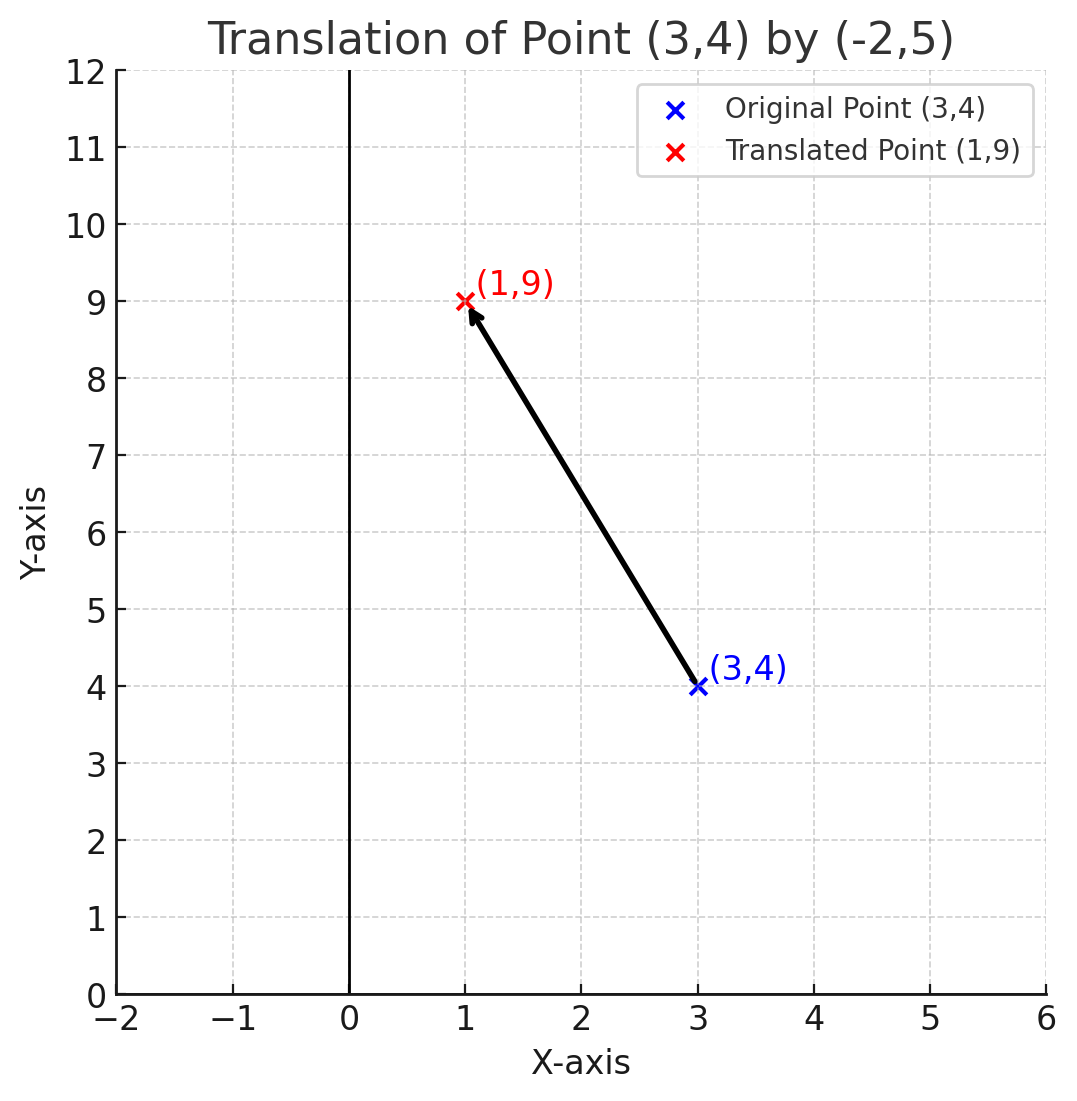
\includegraphics[width=0.6\textwidth]{3.12.png}
	\end{center}
	
	
	Thus, the new coordinates are **$(1,9)$**.
\end{flushleft}

\begin{flushleft}
	\textbf{Example 2: Rotate the point $(2,3)$ by $90^\circ$ counterclockwise about the origin.}
	
	\textbf{Solution:}
	
	Using the $90^\circ$ rotation formula:
	\[
	(x', y') = (-y, x).
	\]
	
	\[
	(x', y') = (-3,2).
	\]
	\begin{center}
		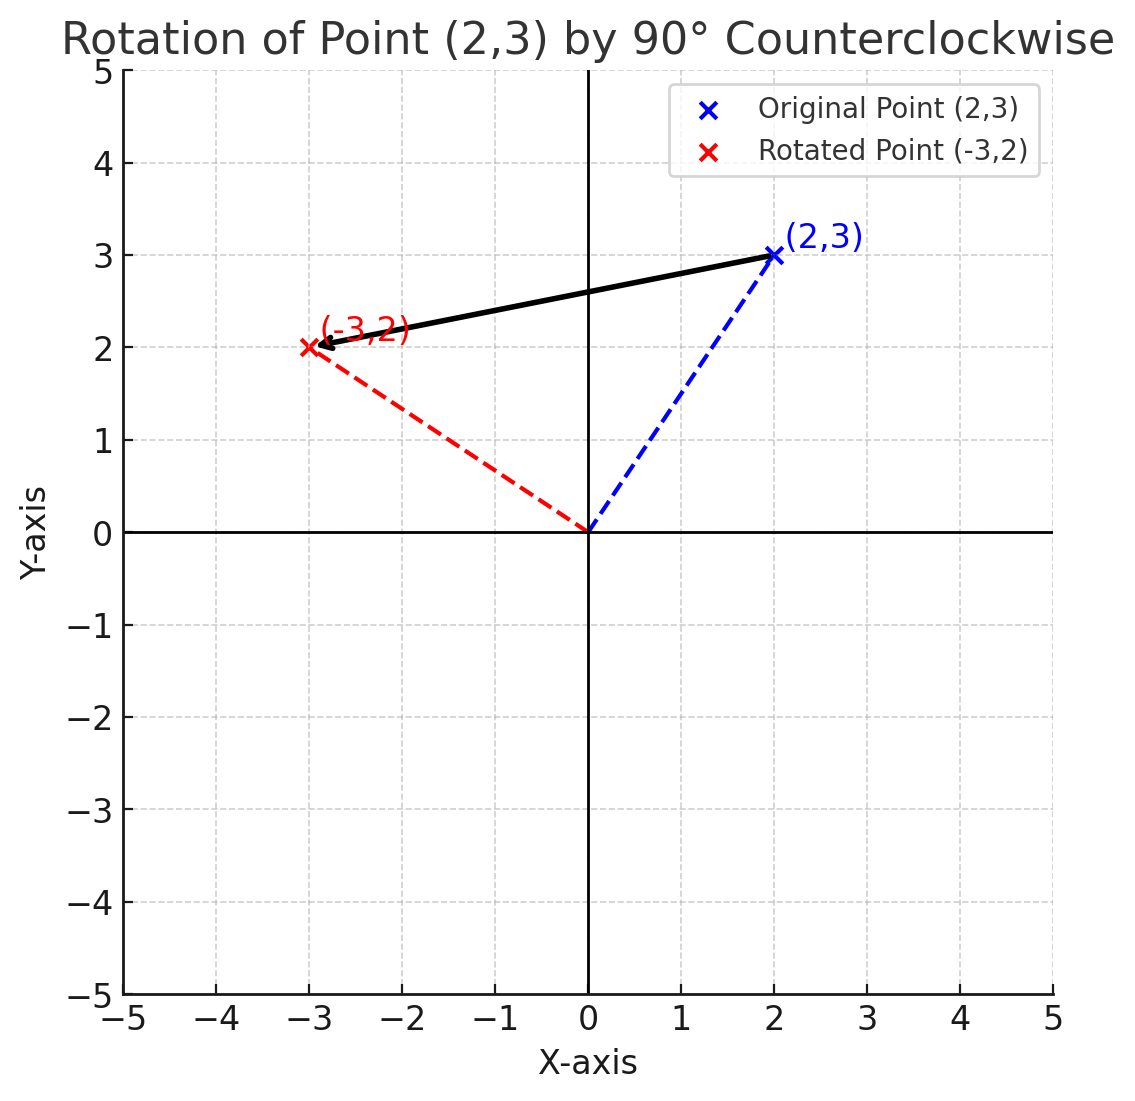
\includegraphics[width=0.6\textwidth]{3.13.png}
	\end{center}
	
	Thus, the new coordinates are **$(-3,2)$**.
\end{flushleft}

\begin{flushleft}
	\textbf{Example 3: Reflect the point $(5, -2)$ across the $y$-axis.}
	
	\textbf{Solution:}
	
	Reflection over the $y$-axis:
	\[
	(x', y') = (-x, y).
	\]
	
	\[
	(x', y') = (-5, -2).
	\]
	\begin{center}
		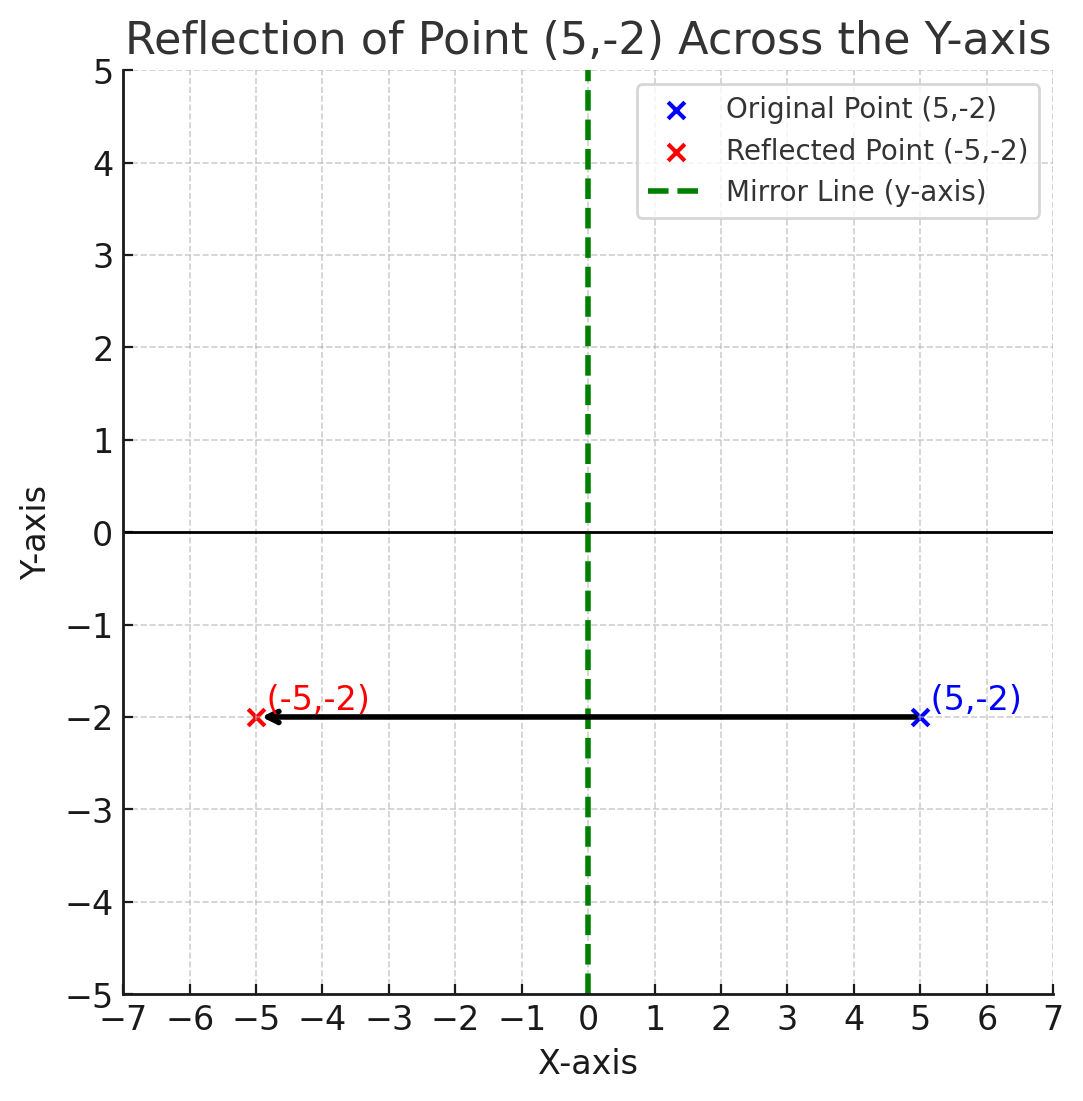
\includegraphics[width=0.6\textwidth]{3.14.png}
	\end{center}
	Thus, the new coordinates are **$(-5,-2)$**.
\end{flushleft}

\begin{flushleft}
	\textbf{Example 4: Enlarge the point $(2, 3)$ by scale factor $k=2$ about the origin.}
	
	\textbf{Solution:}
	
	Using the enlargement formula:
	\[
	(x', y') = (kx, ky).
	\]
	
	\[
	(x', y') = (2 \times 2, 2 \times 3) = (4,6).
	\]
	\begin{center}
		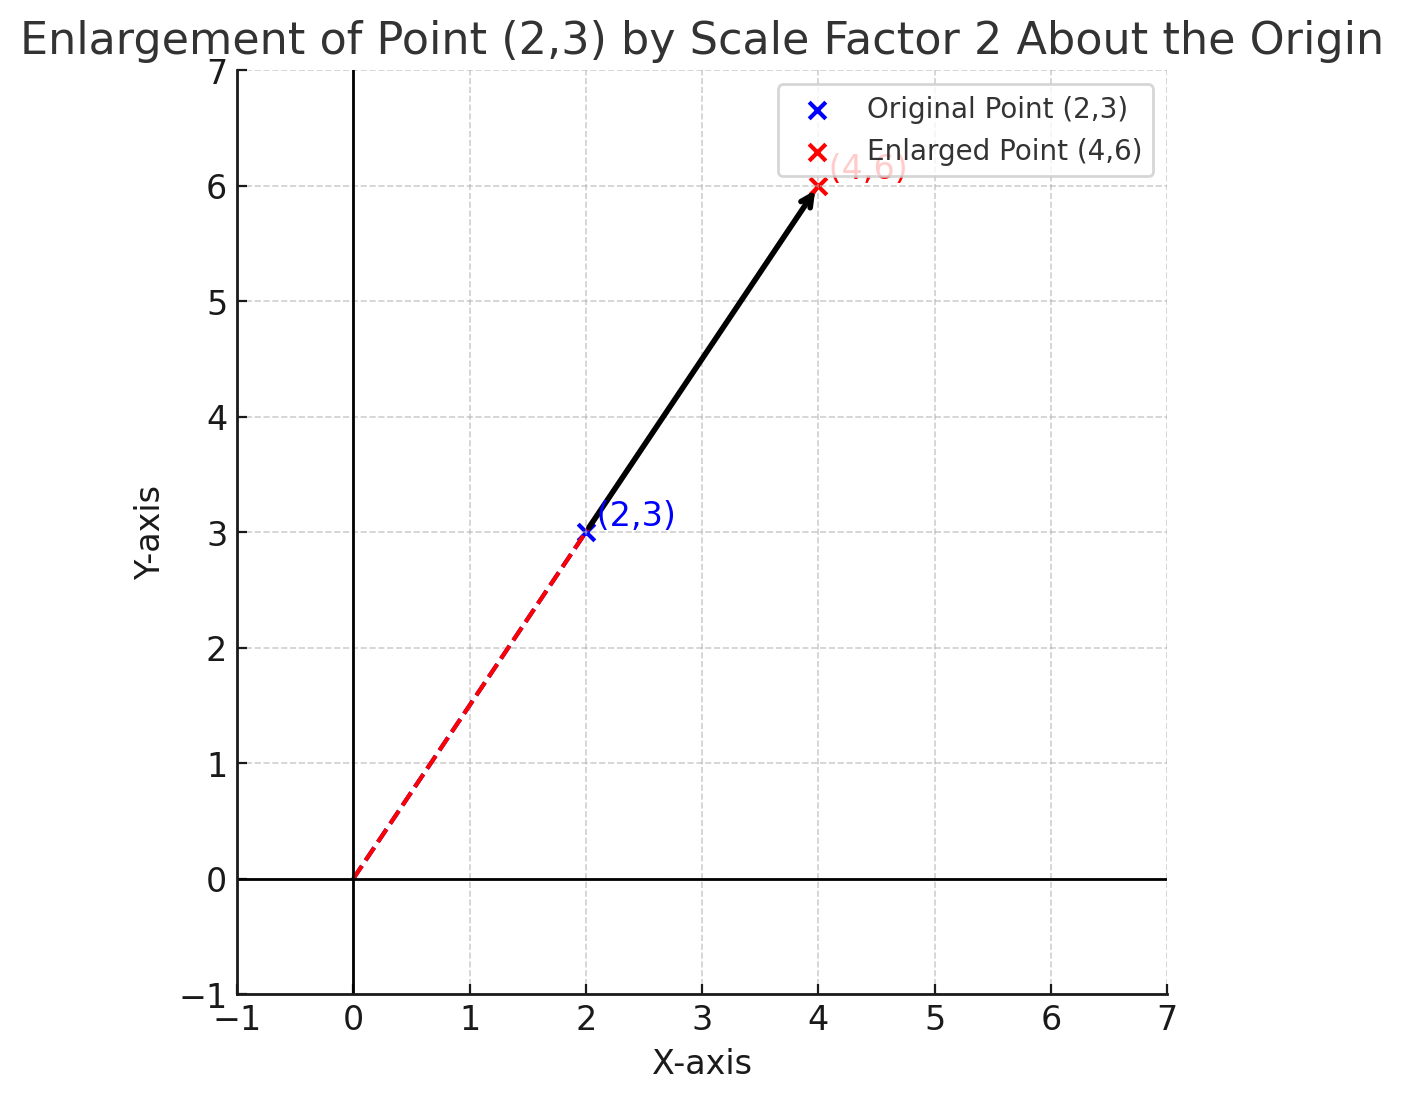
\includegraphics[width=0.6\textwidth]{3.15.png}
	\end{center}
	Thus, the new coordinates are **$(4,6)$**.
\end{flushleft}

\begin{flushleft}
	\textbf{Example 5: Apply a shear transformation with shear factor $k=3$ along the $x$-axis to the point $(1,2)$.}
	
	\textbf{Solution:}
	
	Using the shear formula:
	\[
	(x', y') = (x + ky, y).
	\]
	
	\[
	(x', y') = (1 + 3(2), 2) = (7,2).
	\]
	\begin{center}
		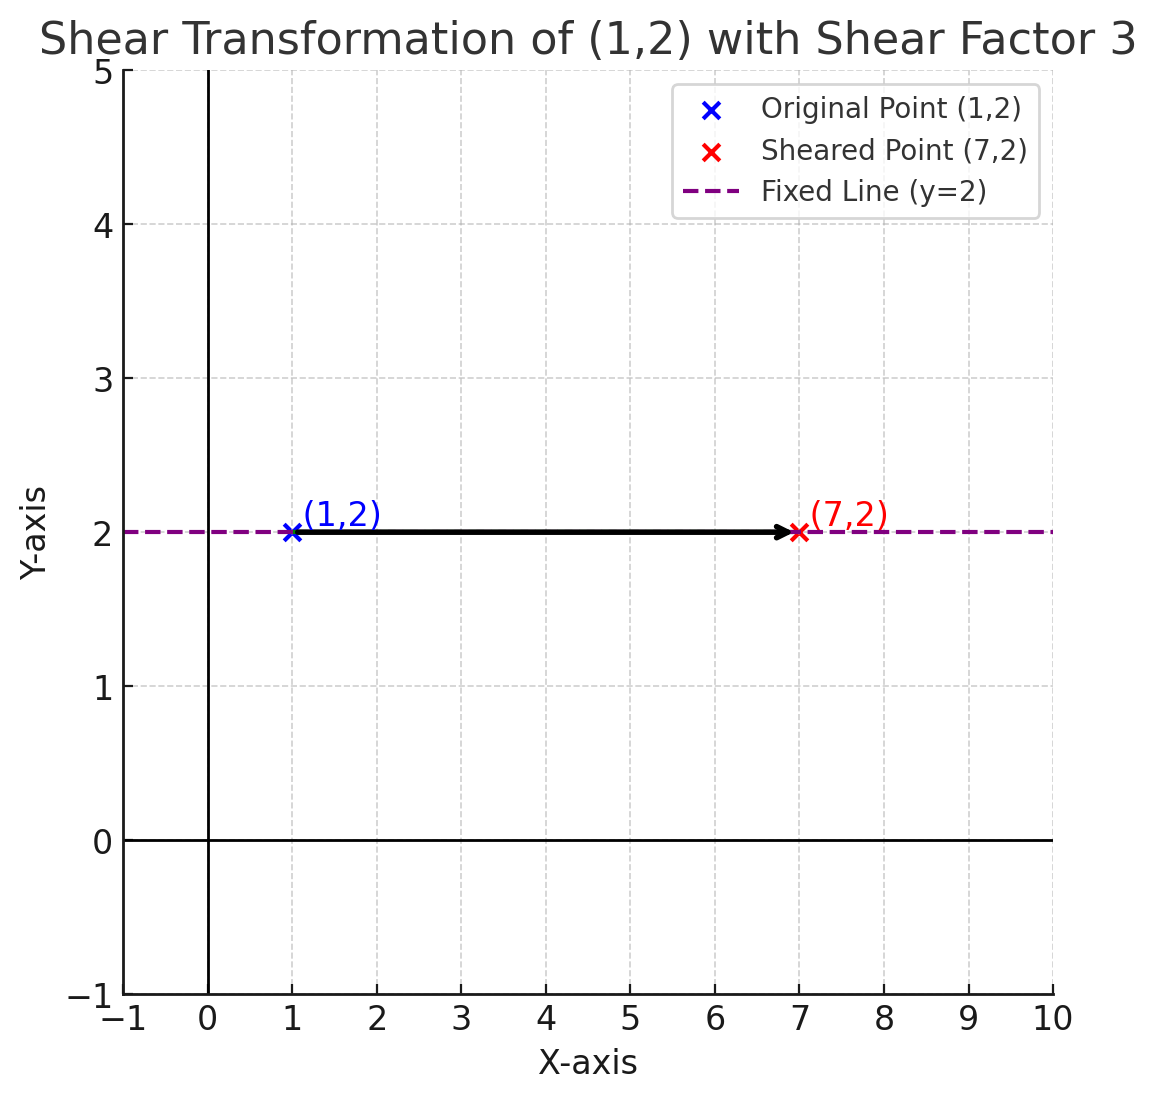
\includegraphics[width=0.6\textwidth]{3.16.png}
	\end{center}
	Thus, the new coordinates are **$(7,2)$**.
\end{flushleft}

